
\title[Python]{Introducción a Python}
\date{}
\author[Fran Rúa/Breixo Camiña]{}
\institute{}

\section{Python}
\label{sec:Python}

\usebackgroundtemplate{}
\begin{frame}
  \titlepage
  \begin{figure}[H]
    \centering
    
\includegraphics[scale=0.5]{python-logo}
  \end{figure}
\end{frame}

\usebackgroundtemplate{%
  \tikz[overlay,remember picture] 
  \node[opacity=0.3 , at=(current page.south east),anchor=south east] {
    
\includegraphics[]{logo-labs}};
}

\begin{frame}
  \frametitle{Fontes e referencias}
  \begin{itemize}
  \item Documentación oficial de Python\\
    {\color{blue}\url{www.python.org/doc}}
  \item Guías de estilo PEP\\
    {\color{blue}\url{www.python.org/dev/peps/pep-0008/}}
  \item Guía para principiantes\\
    {\color{blue}\url{wiki.python.org/moin/BeginnersGuide}}
  \item Learn Python (español)\\
    {\color{blue}\url{http://www.learnpython.org/es/}}
  \item Tracducción do manual de Guido van Rossum
    {\color{blue}\url{http://docs.python.org.ar/tutorial/pdfs/TutorialPython2.pdf}}
  \item Información adiccional\\
    {\color{blue}\url{s.wikipedia.org/wiki/Python}}
  \end{itemize}
\end{frame}

\subsection{Introducción}
\label{subsec:Introduccion}

\begin{frame}
  \frametitle{Introducción}
  \begin{itemize}
  \item Historia
  \item Para qué é usado.
  \item Características
  \item Ventaxas
  \item Inconvintes
  \end{itemize}
\end{frame}

\begin{frame}
  \frametitle{Historia}
  \begin{itemize}
  \item Creado a finais dos 80's por Guido van Rossum
  \item Desenvolvido para o SO Amoeba
  \item Toma partes de outros linguaxes de programación, como Haskell ou ABC
  \item A súa finalidade é programar facilmente e obrigar ó programador a
    realizar código entendible.
  \item Python 1.0 liberado en xaneiro de 1994
  \item Actualmente dous proxectos paralelos: Python 2.7 e Python 3.4
  \item Instalado por defecto na maioría das distribucións GNU/Linux
  \end{itemize}
\end{frame}

\begin{frame}
  \frametitle{Características}
  \begin{itemize}
  \item Linguaxe de programación interpretado
  \item Multiplataforma
  \item Multiparadigma (Programación imperativa, orientada a obxectos e funcional)
  \item Tipado dinámico
  \item Código aberto (Python Software Foundation License, compatible con GNU)
  \item Herencia
  \item Modo interactivo
  \end{itemize}
\end{frame}

\begin{frame}
  \frametitle{Para qué é usado}
  \begin{itemize}
  \item Inicialmente, tareas livianas ou de administración.
  \item Posúe unha ampla cantidade de librerías que posibilita un amplo rango
    de escenarios de uso
  \item Computación numérica
  \item Xeración de gráficos
  \item Programación web
  \item Interacción con bases de datos
  \item Programas de usuario con interface gráfico.
  \end{itemize}
\end{frame}

\subsection{Funcionamento}
\label{subsec:funcionamento}

\begin{frame}
  \frametitle{Funcionamento}
  Ó contrario que C ou Java, Python non precisa ser compilado. En realidade
  Python é un intérprete de comandos que acepta unha serie de instruccións que
  respetan unha serie de normas lóxicas e semánticas.

  Por tanto, se queremos executar o noso código en múltiples plataformas, só é
  necesario instalar o intérprete, xa que despois será éste o encargado de
  executar as órdes indicadas polas instruccións.
\end{frame}

\begin{frame}
  \frametitle{Compilación vs. Interpretación}
  \begin{figure}[ht]
    \centering
    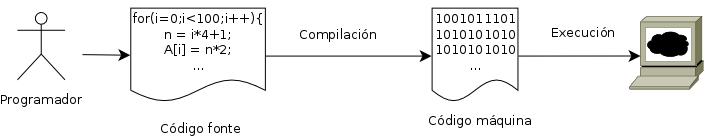
\includegraphics[scale=0.3]{compilacion.png}
    \caption{Compilacion de un programa}
  \end{figure}
\end{frame}

\begin{frame}
  \frametitle{Compilación vs. Interpretación}
  \begin{figure}[ht]
    \centering
    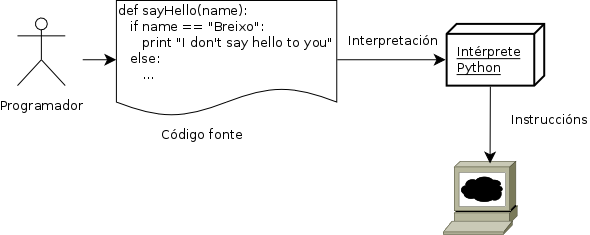
\includegraphics[scale=0.3]{interpretacion.png}
    \caption{Interpretacion de un programa}
  \end{figure}
\end{frame}

\subsection{Modo Interactivo}
\label{subsec:modo interactivo}

\begin{frame}
  \frametitle{Que é o modo interactivo?}
  O modo interactivo permítenos iniciar unha instancia do intérprete de python,
  o que nos permite programar en tempo real e comprobar a sintaxis do noso
  programa.
  
  Neste modo podemos cargar librerías e módulos, ee executar funcións de forma
  rápida sen necesidade de realizar programas previamente.
\end{frame}

\begin{frame}[fragile]
  \frametitle{Iniciar modo interactivo}
  Nos sistemas GNU/Linux soamente é necesario abrir un emulador do terminal e
  escribir \emph{python}.
  \small
\begin{verbatim}
[fran@izanami ~]$ python
Python 2.7.10 (default, Sep 24 2015, 17:50:09) 
[GCC 5.1.1 20150618 (Red Hat 5.1.1-4)] on linux2
Type "help", "copyright", "credits" or "license" for more information.
>>> 
\end{verbatim}
  \normalsize
\end{frame}

\begin{frame}
  \frametitle{Sair do modo interactivo}
  Unha vez que rematemos, para sair do modo iteractivo só temos que chamar á
  función \emph{exit()}

  As funcións e variables definidas nunha sesión do intérprete son borrados unha
  vez que se finaliza dita sesión.
\end{frame}

\subsection{Programando en Python}
\label{subsec:Programando}

\begin{frame}
  \frametitle{Tipos básicos}
  Os tipos de datos básicos definidos por Python son os seguintes:
  \begin{itemize}
  \item Enteiros (int)
  \item Numeros en punto flotante (float)
  \item Números longos (long)
  \item Números en base octal e hexadecimal
  \item Números complexos (complex)
  \item Caracteres (char)
  \item Cadeas de caracteres (string)
  \item tuplas (tuple)
  \end{itemize}
\end{frame}

\begin{frame}
  \frametitle{Operadores lóxicos}
  \begin{itemize}
  \item and, \&
  \item or, $|$
  \item not
  \item is, is not
  \item in, not in
  \end{itemize}
\end{frame}

\begin{frame}
  \frametitle{Operadores matemáticos}
  \begin{itemize}
  \item + (suma)
  \item - (resta)
  \item / (division)
  \item * (multiplicación)
  \item \% (módulo)
    % \item << >> (desplazamiento n bits a dereita ou esquerda)
  \end{itemize}
\end{frame}

\begin{frame}
  \frametitle{Estructuras de datos}
  Ademais dos tipos de datos básicos, Python soporta de forma nativa varias
  estructuras de datos, das cales veremos as dúas máis empregadas.
  \begin{itemize}
  \item \textbf{Listas}\\
    Conxunto de tipos básicos(enteiros, numeros en punto flotante) ou
    compostos(tuplas), poden estar ordenados ou non.\\
    a = [1,2,3,4]
  \item \textbf{Diccionarios}\\
    Asocian un valor a unha clave para mellorar o acceso a un determinado
    elemento.\\
    alumnos = \{'00001A':'Breixo','00002B':'Fran'\}
  \end{itemize}
\end{frame}

\begin{frame}[fragile]
  \frametitle{Definir variables}
  O intérprete python ten incorporado un motor de inferencia, o que significa
  que cando declaramos unha variable non temos que declarar o seu tipo, xa se
  encarga o propio intérprete de inferilo. Se temos dudas acerca do typo de unha
  variable, podemos sabelo coa función \emph{type()}
  \small
\begin{verbatim}
>>> sete = 7
>>> type(sete)
<type 'int'>
>>> a = "primeiro"
>>> type(a)
<type 'str'>
\end{verbatim}
  \normalsize  
\end{frame}

\begin{frame}[fragile]
  \frametitle{Funcións incorporadas (Built-in functions)}
  Python fai uso ten librerías por defecto, que non é necesario cargar, que
  proveen funcionalidades básicas, coma \emph{print()}, que aplicado sobre un
  tipo devolve a súa representación en caracteres.
  \small
\begin{verbatim}
>>> n = "cadea"
>>> print(n)
cadea
>>> numero = 745
>>> print(numero)
745
>>> flotante = 3.14
>>> print(flotante)
3.14
\end{verbatim}
  \normalsize   
\end{frame}

\begin{frame}
  \frametitle{Operacións sobre diccionarios}
  As operacións sobre direccionarios son proporcionados polas librerías básicas,
  xa que son un tipo moi empregado.
  \begin{itemize}
  \item Declaración\\
    d1 = {}
  \item Obter un elemento\\
    d1['clave']
  \item Engadir un elemento\\
    d1.update({'clave':'valor'})
  \item Borrar un elemento\\
    del d1['clave]
  \end{itemize}
\end{frame}

\begin{frame}
  \frametitle{Operacións sobre listas}
  Ó igual que os diccionarios, as listas tamén son moi empregadas e as
  operacións sobre estas son amplamente soportadas.
  \begin{itemize}
  \item Declaración\\
    l = []
  \item Obter un elemento por índice (comeza por 0)\\
    l[7]
  \item Engadir un elemento o final da lista\\
    l.append(n)
  \item Borrar un elemento i\\
    del l[i]
  \end{itemize}
\end{frame}

\begin{frame}[fragile]
  \frametitle{Definir funcións}
  Cando un fragmento de código é executado en numerosas ocasións, ou o código é
  extenso e complexo faise necesario estructuralo en funcións. En python as
  funcións declaranse da seguinte forma:
  \small
\begin{verbatim}
def <nome_funcion>(parametro1,parametro2,...,parametroN):
   sentencias dentro da función
\end{verbatim}  
  \normalsize
\end{frame}

\begin{frame}[fragile]
  \frametitle{Función de suma}
  \small
\begin{verbatim}
>>> def suma(a,b):
...    return a+b
... 
>>> suma(3,4)
7
\end{verbatim}
\end{frame}

\begin{frame}[fragile]
  \frametitle{Indentación}
  Como vimos ó principio, un dos obxectivos de Python é conseguir un código
  claro e lexible, para o cal fai obligatorio o uso da indentación.

  Unha mala indentación cambia o significado do programa.
  \begin{multicols}{2}
    \begin{lstlisting}
      def access_control(name, pass):
        if authentication(name,pass) == 0:
          print(``Access denied'')
          exit()
        else:
          print(``Access granted'')
          grant_access()
    \end{lstlisting}
    \columnbreak
    \begin{lstlisting}
      def access_control(name, pass):
        if authentication(name,pass) == 0:
          print(``Access denied'')
          exit()
        else:
          print(``Access granted'')
        grant_access()
    \end{lstlisting}
  \end{multicols}
\end{frame}

\begin{frame}[fragile]
  \frametitle{Estructuras de control}
  \framesubtitle{If}
  \small
  \begin{verbatim}
    if (test1):
       print a
    elif (test2 and test3):
       print b
       exit()
    elif (test4):
       print(``nada que facer'')
    else:
       print(``Saindo'')
  \end{verbatim}
  \normalsize
\end{frame}

\begin{frame}[fragile]
  \frametitle{Estructuras de control}
  \framesubtitle{Bucle for}
  Os bucles for son aplicados sobre listas. Esto quere decir que se queremos
  percorrer unha lista e aplicar unha función a cada elemento, ésto é posible
  mediante o seguinte código
  \small
\begin{verbatim}
>>> alumnos = ["Xoan", "Marcos","Jesus", "Bea"]
>>> for alumno in alumnos:
...    print alumno
... 
Xoan
Marcos
Jesus
Bea
>>> 
\end{verbatim}
  \normalsize
\end{frame}

\begin{frame}[fragile]
  \frametitle{Bucle for}
  Se queremos un bucle secuencial, podemos empregar a función \emph{range}, que
  crea unha lista de elementos.
  \small
  \begin{verbatim}
    >>> for n in range(2,8):
    ...    print n
    ... 
    2
    3
    4
    5
    6
    7
    >>> 
  \end{verbatim}
  \normalsize
\end{frame}

\begin{frame}[fragile]
  \frametitle{Estructuras de control}
  \framesubtitle{Bucle while}
  Igual que no resto de linguaxes de programación, o bucle while permítenos
  realizar unha acción repetitiva mentrs se cumpla unha condición, usando a a
  sentencia \textbf{break} para saír. Se non queremos saír do bucle, senón
  saltar as sentencias pendentes e executar o seguinte salto de bucle usamos
  \textbf{continue}.
  \small
\begin{verbatim}
    while(true):
       if(test1):
          continue
       elif(test2):
          print("Hola")
       else:
          break    
\end{verbatim}
  \normalsize
\end{frame}

\begin{frame}
  \frametitle{Ficheiros de código}
  Python é un programa de scripting, é decir, as instruccións son escritas nun
  ficheiro de texto plano, con extensión \emph{.py} tal e como serían
  introducidas no intérprete.  

  A execución de un script consiste básicamente na lectura secuencial do
  ficheiro de texto e a execución das insctruccións correspondentes por parte do
  intérprete. 

  Existen dous tipos de programar en ficheiros: módulos e programas.
\end{frame}

\begin{frame}
  \frametitle{Módulos}
  Os módulos son definicións de funcións. Se existen funcións que usamos
  reiteradamente, podemos definilas nun ficheiro con extensión \emph{.py} e
  importalo despois mediante a orde \textbf{import}.

  Os módulos proporcionan funcionalidades, pero non realizan accións de por sí,
  senon que son usados polos programas para axilizar o desenvolvemento de
  aplicacións. 

  Existen dúas formas de referenciar módulos, \textbf{import} e \textbf{from}
\end{frame}

\begin{frame}[fragile]
  \frametitle{Modulo operacions.py}
  \small
  \begin{verbatim}
    def suma (a,b):
        return a+b
    
    def resta (a,b):
        return a-b

    def devolve_maior (a,b):
        if (a>b):
            return a
        else:
            return b
  \end{verbatim}
  \normalsize
\end{frame}

\begin{frame}[fragile]
  \frametitle{import}
  A sentencia \textbf{import} carga todas as funcións do módulo ó que
  referenciamos, o cal pode ser ineficiente se non as empregamos.

  Ademáis, o programador debe especificar o espazo de nomes, é decir,
  referenciar o módulo ó que pertence a función que queremos empregar.

  \small
  \begin{verbatim}
>>> import operacions
>>> suma(2,8)
Traceback (most recent call last):
  File "<stdin>", line 1, in <module>
NameError: name 'suma' is not defined
>>> operacions.suma(2,8)
10
  \end{verbatim}  
  \normalsize
\end{frame}

\begin{frame}[fragile]
  \frametitle{from}
  Mediante a orde \textbf{from}, podemos importar funcións concretas de un
  módulo e, ademáis, importar o seu espazo de nomes, polo que non é necesario
  facer referencia ó módulo ó que pertence.
  \small
  \begin{verbatim}
>>> from operacions import devolve_maior
>>> devolve_maior(15,8)
15
>>> operacions.devolve_maior(15,8)
Traceback (most recent call last):
  File "<stdin>", line 1, in <module>
NameError: name 'operacions' is not defined
  \end{verbatim}
  \normalsize
\end{frame}

\begin{frame}
  \frametitle{Scripts Python}
  Obviamente é interesante ter programas que se executen de forma que non sexa
  necesario o uso de unha sesión interactiva co intérprete. A estes ficheiros
  denomínase scripts, e, ó igual que os módulos, son leidos polo intérprete de
  forma secuencial.

  Neles podemos definir un conxunto de funcións e variables coas que construir
  unha secuencia de pasos a executar.

  Para que se execute é necesario que exista unha función \textbf{main}, que é a
  última en ser declarada.

  Cando o intérprete lee un arquivo de texto, se existe unha función main
  executa as ordes dentro dela como si se tratara dunha sesión interactiva, de
  forma que pode ser usada como disparador de un conxunto de accións.
\end{frame}

\begin{frame}[fragile]
  \frametitle{Cabeceiras}
  Para executar un programa en python, tan só é necesario asegurarnos de que o
  arquivo ten permisos de execución e a continuación chamar ó interprete sobre o
  ficheiro.
  \small
  \begin{verbatim}
    python arquivo.py
  \end{verbatim}
  \normalsize
  É posible engadir a seguinte liña para que o script sexa executado polo propio
  entorno de usuario.
  \small
  \begin{verbatim}
    #!/usr/bin/env python 
  \end{verbatim}
  \normalsize
  Tamén é recomendable, se o texto vai incluir carácteres que poden ser
  problemáticos coma 'ñ', ou tildes, especificar a codificación na que se gardou
  o ficheiro. O máis apropiado é facelo en UTF-8
  \begin{verbatim}
    # -*- coding: utf-8 -*-
  \end{verbatim}
  \normalsize
\end{frame}

\begin{frame}
  \frametitle{Inconvintes}
  \begin{itemize}
  \item Os erros teñen lugar en tempo de execución
  \item Como o tipado é dinamico, require que o programador preste maior
    atención a estos detalles.
  \item Rendemento, principalmente na carga de código
  \end{itemize}
\end{frame}